\begin{figure}[H]
    \begin{center}
        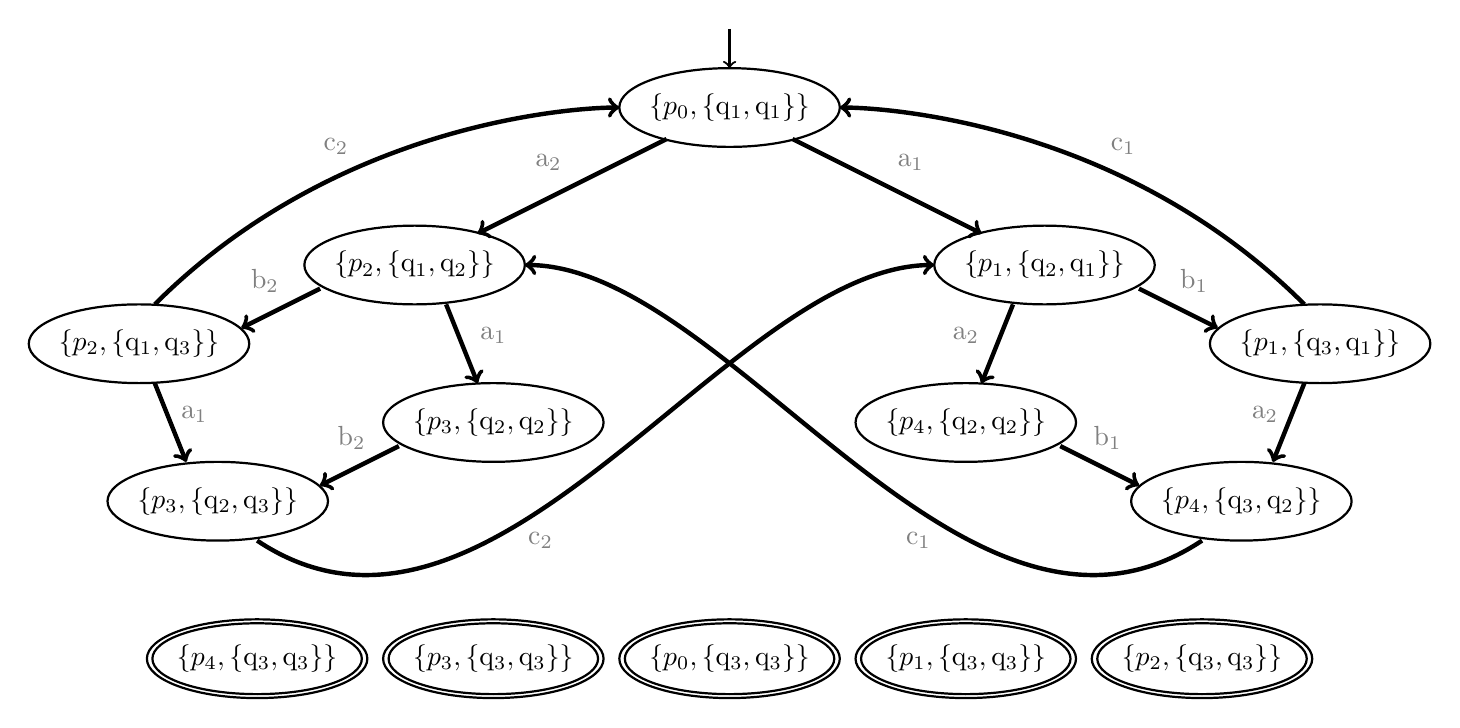
\begin{tikzpicture}
        
        %Ellipses
        %Top layer
        \draw[thick] (0,0) ellipse (1.4 and 0.5) node {$\{p_0, \{\mathrm{q_1,q_1}\}\}$};
        
        %Layer 1
        %left
        \draw[thick] (-4,-2) ellipse (1.4 and 0.5) node {$\{p_2, \{\mathrm{q_1,q_2}\}\}$};
        %right
        \draw[thick] (4,-2) ellipse (1.4 and 0.5) node {$\{p_1, \{\mathrm{q_2,q_1}\}\}$};
        
        %Layer 2
        %left 0
        \draw[thick] (-7.5,-3) ellipse (1.4 and 0.5) node {$\{p_2, \{\mathrm{q_1,q_3}\}\}$};    
        %left 1
        \draw[thick] (-3,-4) ellipse (1.4 and 0.5) node {$\{p_3, \{\mathrm{q_2,q_2}\}\}$};
    
        %right 0
        \draw[thick] (7.5,-3) ellipse (1.4 and 0.5) node {$\{p_1, \{\mathrm{q_3,q_1}\}\}$};
        %right 1
        \draw[thick] (3,-4) ellipse (1.4 and 0.5) node {$\{p_4, \{\mathrm{q_2,q_2}\}\}$};
        
        %Layer 3
        %left        
        \draw[thick] (-6.5,-5) ellipse (1.4 and 0.5) node {$\{p_3, \{\mathrm{q_2,q_3}\}\}$};
        %right        
        \draw[thick] (6.5,-5) ellipse (1.4 and 0.5) node {$\{p_4, \{\mathrm{q_3,q_2}\}\}$};
        
        %Layer 4 (Final states)
        \draw[thick] (0,-7) ellipse (1.4 and 0.5) node {$\{p_0, \{\mathrm{q_3,q_3}\}\}$};
        \draw[thick] (0,-7) ellipse (1.33 and 0.45);
        
        \draw[thick] (3,-7) ellipse (1.4 and 0.5) node {$\{p_1, \{\mathrm{q_3,q_3}\}\}$};
        \draw[thick] (3,-7) ellipse (1.33 and 0.45);
        
        \draw[thick] (6,-7) ellipse (1.4 and 0.5) node {$\{p_2, \{\mathrm{q_3,q_3}\}\}$};
        \draw[thick] (6,-7) ellipse (1.33 and 0.45);
        
        \draw[thick] (-3,-7) ellipse (1.4 and 0.5) node {$\{p_3, \{\mathrm{q_3,q_3}\}\}$};
        \draw[thick] (-3,-7) ellipse (1.33 and 0.45);
        
        \draw[thick] (-6,-7) ellipse (1.4 and 0.5) node {$\{p_4, \{\mathrm{q_3,q_3}\}\}$};
        \draw[thick] (-6,-7) ellipse (1.33 and 0.45);
        
        
        %Edges
        
        %Initial edge
        \draw[thick, ->] (0,1)--(0,0.5);
        
        %left diamond
        \draw[ultra thick,->] (-0.8,-0.4) -- (-3.2,-1.6); 
        
        \draw[ultra thick,->] (-5.2,-2.3) -- (-6.2,-2.8); 
        
        \draw[ultra thick,->] (-3.6,-2.5) -- (-3.2,-3.5); 
        
        \draw[ultra thick,->] (-4.2,-4.3) -- (-5.2,-4.8); 
        
        \draw[ultra thick,->] (-7.3,-3.5) -- (-6.9,-4.5); 
        
        \draw[ultra thick,->] (-7.3,-2.5) .. controls (-5,-0.2) and (-2,0) .. (-1.4,0);
        
        \draw[ultra thick,->] (-6,-5.5) .. controls (-3,-7.5) and (0,-2) .. (2.6,-2);
        
        %right diamond
        \draw[ultra thick,->] (0.8,-0.4) -- (3.2,-1.6); 
        
        \draw[ultra thick,->] (5.2,-2.3) -- (6.2,-2.8); 
        
        \draw[ultra thick,->] (3.6,-2.5) -- (3.2,-3.5); 
        
        \draw[ultra thick,->] (4.2,-4.3) -- (5.2,-4.8);
        
        \draw[ultra thick,->] (7.3,-3.5) -- (6.9,-4.5); 
        
        \draw[ultra thick,->] (7.3,-2.5) .. controls (5,-0.2) and (2,0) .. (1.4,0);
        
        \draw[ultra thick,->] (6,-5.5) .. controls (3,-7.5) and (0,-2) .. (-2.6,-2);
        
        
        
        %Labels
        %left diamond
        \draw[gray] (-2.3,-0.7) node {$\mathrm{a_2}$};
        \draw[gray] (-5.9,-2.2) node {$\mathrm{b_2}$};
        \draw[gray] (-3,-2.9) node {$\mathrm{a_1}$};
        \draw[gray] (-4.8,-4.2) node {$\mathrm{b_2}$};
        \draw[gray] (-6.8,-3.9) node {$\mathrm{a_1}$};
        \draw[gray] (-5,-0.5) node {$\mathrm{c_2}$};
        \draw[gray] (-2.4,-5.5) node {$\mathrm{c_2}$};
        
                
        %right diamond
        \draw[gray] (2.3,-0.7) node {$\mathrm{a_1}$};
        \draw[gray] (5.9,-2.2) node {$\mathrm{b_1}$};
        \draw[gray] (3,-2.9) node {$\mathrm{a_2}$};
        \draw[gray] (4.8,-4.2) node {$\mathrm{b_1}$};
        \draw[gray] (6.8,-3.9) node {$\mathrm{a_2}$};
        \draw[gray] (5,-0.5) node {$\mathrm{c_1}$};
        \draw[gray] (2.4,-5.5) node {$\mathrm{c_1}$};
        
        
        \end{tikzpicture}
    \end{center}
    \caption{The product automaton for the intersection between $\mathcal{L}(\mathbf{M})$ and $\mathcal{L}(\mathbf{T})$ (dead state and non-reachable states not shown). None of the machine's final states are reachable from its initial state, and are therefore shown isolated below, with no edges.}
    \label{fig:MxT}
\end{figure}
